\documentclass[tikz,border=10pt]{standalone}
\usepackage{amsmath,amssymb}
\usepackage{tikz}
\usetikzlibrary{arrows.meta,calc,positioning}

\definecolor{navy}{HTML}{1B365D}
\definecolor{steelblue}{HTML}{2471A3}
\definecolor{teal}{HTML}{0E6251}
\definecolor{amber}{HTML}{D35400}
\definecolor{crimson}{HTML}{C0392B}
\definecolor{slate}{HTML}{566573}
\definecolor{purple}{HTML}{6C3483}

\begin{document}
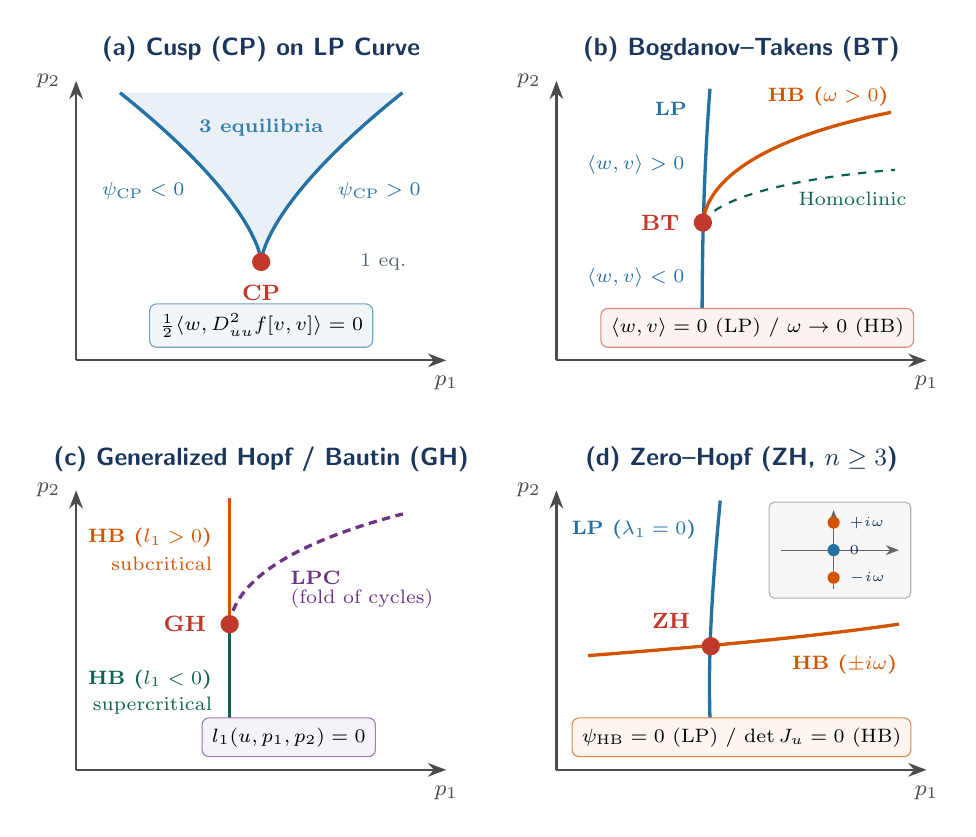
\begin{tikzpicture}[
    >=Stealth,
    font=\sffamily\small,
]

% ========================
% PANEL (a): Cusp (CP) on LP curve
% ========================
\begin{scope}[shift={(0, 5.2)}]
    \node[font=\sffamily\bfseries\small, navy] at (2.55, 4.35)
        {(a) Cusp (CP) on LP Curve};

    % Axes
    \draw[->, thick, black!70] (0.2, 0.4) -- (4.9, 0.4) node[below=2pt, font=\footnotesize] {$p_1$};
    \draw[->, thick, black!70] (0.2, 0.4) -- (0.2, 3.95) node[left=2pt, font=\footnotesize] {$p_2$};

    % Shaded 3-equilibria wedge
    \fill[steelblue!10]
        plot[domain=0:1.05, samples=40] ({2.55 + 1.55*\x*\x*\x}, {1.65 + 1.95*\x*\x})
        -- plot[domain=1.05:0, samples=40] ({2.55 - 1.55*\x*\x*\x}, {1.65 + 1.95*\x*\x}) -- cycle;

    % Two LP branches meeting at cusp
    \draw[very thick, steelblue, domain=0:1.05, samples=50]
        plot ({2.55 - 1.55*\x*\x*\x}, {1.65 + 1.95*\x*\x});
    \draw[very thick, steelblue, domain=0:1.05, samples=50]
        plot ({2.55 + 1.55*\x*\x*\x}, {1.65 + 1.95*\x*\x});

    % Cusp point
    \fill[crimson] (2.55, 1.65) circle (3.3pt);
    \node[crimson, font=\footnotesize\bfseries, below=4pt] at (2.55, 1.62) {CP};

    % Region & sign annotations
    \node[steelblue!90, font=\scriptsize\bfseries] at (2.55, 3.35) {3 equilibria};
    \node[slate, font=\scriptsize] at (4.10, 1.65) {1 eq.};
    \node[steelblue, font=\scriptsize, anchor=east] at (1.70, 2.55) {$\psi_{\mathrm{CP}} < 0$};
    \node[steelblue, font=\scriptsize, anchor=west] at (3.40, 2.55) {$\psi_{\mathrm{CP}} > 0$};

    % Condition box
    \node[draw=steelblue!65, fill=steelblue!6, rounded corners=2.5pt, font=\scriptsize, anchor=south, inner sep=3.5pt]
        at (2.55, 0.56) {$\frac{1}{2}\langle w, D^2_{uu}f[v,v]\rangle = 0$};
\end{scope}

% ========================
% PANEL (b): Bogdanov-Takens (BT)
% ========================
\begin{scope}[shift={(6.1, 5.2)}]
    \node[font=\sffamily\bfseries\small, navy] at (2.55, 4.35)
        {(b) Bogdanov--Takens (BT)};

    % Axes
    \draw[->, thick, black!70] (0.2, 0.4) -- (4.9, 0.4) node[below=2pt, font=\footnotesize] {$p_1$};
    \draw[->, thick, black!70] (0.2, 0.4) -- (0.2, 3.95) node[left=2pt, font=\footnotesize] {$p_2$};

    % LP curve
    \draw[very thick, steelblue] (2.05, 0.95) .. controls (2.05, 1.95) and (2.08, 2.95) .. (2.15, 3.85);
    \node[steelblue, font=\scriptsize\bfseries, anchor=east] at (1.98, 3.60) {LP};

    % HB curve tangent to LP at BT (upper half only)
    \draw[very thick, amber] (2.06, 2.15) .. controls (2.12, 2.75) and (2.95, 3.25) .. (4.45, 3.55);
    \node[amber, font=\scriptsize\bfseries, anchor=south] at (3.65, 3.50) {HB ($\omega > 0$)};

    % Homoclinic curve tangent to LP/HB
    \draw[thick, teal, dashed] (2.06, 2.15) .. controls (2.25, 2.48) and (3.25, 2.72) .. (4.50, 2.82);
    \node[teal, font=\scriptsize, anchor=north west] at (3.15, 2.66) {Homoclinic};

    % BT point
    \fill[crimson] (2.06, 2.15) circle (3.3pt);
    \node[crimson, font=\footnotesize\bfseries, left=5pt] at (2.06, 2.15) {BT};

    % Sign of <w, v> along LP
    \node[steelblue, font=\scriptsize, anchor=east] at (1.95, 2.88) {$\langle w, v\rangle > 0$};
    \node[steelblue, font=\scriptsize, anchor=east] at (1.95, 1.45) {$\langle w, v\rangle < 0$};

    % Condition box
    \node[draw=crimson!60, fill=crimson!6, rounded corners=2.5pt, font=\scriptsize, anchor=south, inner sep=3.5pt]
        at (2.75, 0.56) {$\langle w,v\rangle = 0$ (LP) / $\omega \to 0$ (HB)};
\end{scope}

% ========================
% PANEL (c): Generalized Hopf / Bautin (GH)
% ========================
\begin{scope}[shift={(0, 0)}]
    \node[font=\sffamily\bfseries\small, navy] at (2.55, 4.35)
        {(c) Generalized Hopf / Bautin (GH)};

    % Axes
    \draw[->, thick, black!70] (0.2, 0.4) -- (4.9, 0.4) node[below=2pt, font=\footnotesize] {$p_1$};
    \draw[->, thick, black!70] (0.2, 0.4) -- (0.2, 3.95) node[left=2pt, font=\footnotesize] {$p_2$};

    % HB curve split into supercritical (teal) and subcritical (amber)
    \draw[very thick, teal] (2.15, 0.95) -- (2.15, 2.25);
    \draw[very thick, amber] (2.15, 2.25) -- (2.15, 3.85);
    \node[teal, font=\scriptsize\bfseries, anchor=east] at (2.05, 1.55) {HB ($l_1 < 0$)};
    \node[teal, font=\scriptsize, anchor=east] at (2.05, 1.22) {supercritical};
    \node[amber, font=\scriptsize\bfseries, anchor=east] at (2.05, 3.35) {HB ($l_1 > 0$)};
    \node[amber, font=\scriptsize, anchor=east] at (2.05, 3.02) {subcritical};

    % LPC curve tangent to HB at GH
    \draw[very thick, purple, densely dashed] (2.15, 2.25) .. controls (2.22, 2.82) and (3.00, 3.30) .. (4.35, 3.65);
    \node[purple, font=\scriptsize\bfseries, align=left, anchor=north west] at (2.80, 3.05) {LPC\\[-1pt]\normalfont\scriptsize (fold of cycles)};

    % GH point
    \fill[crimson] (2.15, 2.25) circle (3.3pt);
    \node[crimson, font=\footnotesize\bfseries, left=5pt] at (2.15, 2.25) {GH};

    % Condition box
    \node[draw=purple!65, fill=purple!6, rounded corners=2.5pt, font=\scriptsize, anchor=south, inner sep=3.5pt]
        at (2.90, 0.56) {$l_1(u, p_1, p_2) = 0$};
\end{scope}

% ========================
% PANEL (d): Zero-Hopf (ZH) for n >= 3
% ========================
\begin{scope}[shift={(6.1, 0)}]
    \node[font=\sffamily\bfseries\small, navy] at (2.55, 4.35)
        {(d) Zero--Hopf (ZH, $n \ge 3$)};

    % Axes
    \draw[->, thick, black!70] (0.2, 0.4) -- (4.9, 0.4) node[below=2pt, font=\footnotesize] {$p_1$};
    \draw[->, thick, black!70] (0.2, 0.4) -- (0.2, 3.95) node[left=2pt, font=\footnotesize] {$p_2$};

    % LP curve
    \draw[very thick, steelblue] (2.15, 1.05) .. controls (2.12, 2.00) and (2.20, 2.95) .. (2.28, 3.82);
    \node[steelblue, font=\scriptsize\bfseries, anchor=east] at (2.10, 3.45) {LP ($\lambda_1 = 0$)};

    % HB curve crossing transversally
    \draw[very thick, amber] (0.60, 1.85) .. controls (1.85, 1.95) and (3.15, 2.05) .. (4.55, 2.25);
    \node[amber, font=\scriptsize\bfseries, anchor=north east] at (4.65, 1.98) {HB ($\pm i\omega$)};

    % ZH point
    \fill[crimson] (2.16, 1.97) circle (3.3pt);
    \node[crimson, font=\footnotesize\bfseries, above left=3pt and 4pt] at (2.16, 1.97) {ZH};

    % Inset eigenvalue mini-plane in upper right (clear of all curves/boxes)
    \begin{scope}[shift={(2.90, 2.58)}]
        \draw[draw=slate!50, fill=slate!5, rounded corners=2pt] (0, 0) rectangle (1.80, 1.22);
        \draw[->, thin, black!60] (0.15, 0.61) -- (1.65, 0.61);
        \draw[->, thin, black!60] (0.82, 0.12) -- (0.82, 1.12);
        \fill[steelblue] (0.82, 0.61) circle (2.2pt);
        \fill[amber] (0.82, 0.96) circle (2.2pt);
        \fill[amber] (0.82, 0.26) circle (2.2pt);
        \node[font=\tiny, navy, anchor=west] at (0.90, 0.96) {$+i\omega$};
        \node[font=\tiny, navy, anchor=west] at (0.90, 0.61) {$0$};
        \node[font=\tiny, navy, anchor=west] at (0.90, 0.26) {$-i\omega$};
    \end{scope}

    % Condition box
    \node[draw=amber!70, fill=amber!6, rounded corners=2.5pt, font=\scriptsize, anchor=south, inner sep=3.5pt]
        at (2.55, 0.56) {$\psi_{\mathrm{HB}}=0$ (LP) / $\det J_u = 0$ (HB)};
\end{scope}

\end{tikzpicture}
\end{document}
